\documentclass[pdf]{beamer}

\usetheme{Warsaw}

\usepackage{alltt}

\usepackage{amssymb, amsmath}

\usepackage[english]{babel}

\usepackage{tikz}
\usetikzlibrary{calc,trees,positioning,arrows,chains,automata,shapes.geometric,%
    decorations.pathreplacing,decorations.pathmorphing,shapes,%
    matrix,shapes.symbols}

\usetikzlibrary{shapes,arrows,automata,positioning,calc}
\usetikzlibrary{fit,backgrounds}
\usetikzlibrary{decorations.pathreplacing}
\tikzset{
>=stealth',
  punktchain/.style={
    rectangle,
    rounded corners,
    % fill=black!10,
    draw=black, very thick,
    text width=6em,
    minimum height=3em,
    text centered,
    on chain},
  line/.style={draw, thick, <-},
  element/.style={
    tape,
    top color=white,
    bottom color=blue!50!black!60!,
    minimum width=8em,
    draw=blue!40!black!90, very thick,
    text width=10em,
    minimum height=3.5em,
    text centered,
    on chain},
  every join/.style={->, thick,shorten >=1pt},
  decoration={brace},
  tuborg/.style={decorate},
  tubnode/.style={midway, right=2pt},
}

% collection of macros used in the paper

%Learners
\newcommand{\learnlib}{LearnLib}

\newcommand{\A}{{\mathcal A}}
\newcommand{\B}{{\mathcal B}}
\newcommand{\CH}{{\mathcal H}}
\newcommand{\M}{{\mathcal M}}
\newcommand{\N}{{\mathcal N}}
\newcommand{\hypoof}[2]{\mathcal{H}(#1,#2)}

\newcommand{\nat}{{\mathbb N}}
\newcommand{\integers}{{\mathbb Z}}

\newcommand{\sem}[1]{[\kern-.5mm[{#1}]\kern-.5mm]}
\newcommand{\eqclass}[1]{[{#1}]}

%DOMAIN AND RANGE
\newcommand{\dom}{{\textsf{dom}}}
\newcommand{\ran}{{\textsf{ran}}}

\newcommand{\natplus}{\nat^{>0}}
\newcommand{\realsplus}{{\mathbb R}^{\geq 0}}
\newcommand{\delays}{{\mathbb R}^{> 0}}
\newcommand{\stoptimer}{\mathit{kill}}
\newcommand{\tosymbol}{\mathit{to}}
\newcommand{\toevent}[1]{\mathit{to}[#1]}
\newcommand{\toevents}{\mbox{\sl TO}}
\newcommand{\extinputs}{\hat{I}}
\newcommand{\Head}[1]{\mathsf{Head}({#1})}
\newcommand{\Tail}[1]{\mathsf{Tail}({#1})}
\newcommand{\Last}[1]{\mathsf{Last}({#1})}
\newcommand{\expirable}{\mathit{expirable}}
\newcommand{\tvals}{\kappa}
\newcommand{\Vals}[1]{\mathit{Val}({#1})}
\newcommand{\delay}[2]{d_{[#1:#2]}}
\newcommand{\timerof}[2]{x_{#1}^{#2}}
\newcommand{\Post}{\mathsf{Post}}
\newcommand{\beh}{\mathit{beh}}
\newcommand{\untime}{\mathit{untime}}
\newcommand{\run}{\mathit{pullback}}
\newcommand{\timedword}{\mathit{tw}}
\newcommand{\timedinputword}{\mathit{tiw}}
\newcommand{\untimedinputword}{\mathit{uiw}}
\newcommand{\startedby}{\mathit{startedby}}
\newcommand{\Mealy}{\mathit{Mealy}}
\newcommand{\finitesubsets}[1]{{\mathcal{P}}_{\mathit{fin}}(#1)}
\newcommand{\conc}{\cdot}
\newcommand{\tuple}[1]{\langle #1\rangle}
\newcommand{\set}[1]{\lbrace #1\rbrace}
\newcommand{\vect}[2]{{#1}_1 , \ldots , {#1}_{#2}}
\newcommand{\setcomp}[2]{\set{#1 ~:~ #2}}
\newcommand{\domof}[1]{\dom(#1)}
\newcommand{\ranof}[1]{\ran(#1)}
\newcommand{\can}[1]{\mathit{can}({#1})}
\newcommand{\uncan}[1]{\mathit{uncan}({#1})}
\newcommand{\zone}[1]{\mathit{Zone}({#1})}
\newcommand{\vars}{\mathcal{X}}
\newcommand{\varsof}[1]{\vars(#1)}
\newcommand{\remap}{\pi}
\newcommand{\remapinst}{\rho}
\newcommand{\constr}{\phi}


\newcommand{\emptyword}{\epsilon}
\newcommand{\lengthof}[1]{|#1|}
\newcommand{\true}{{\it true}}
\newcommand{\false}{{\it false}}

%% macros for ``approximation''
\newcommand{\acttimers}{\mathit{active}}
\newcommand{\constrof}[1]{\phi_{#1}}
\newcommand{\post}{\mathit{post}}

\newcommand{\ctimers}{X}
\newcommand{\normalize}{\gamma}
\newcommand{\normalizeof}[2]{\normalize_{#2}^{#1}}
\newcommand{\timerbij}{\gamma}
\newcommand{\timerequiv}{\pi}
\newcommand{\extendedby}{\lhd}
\newcommand{\uttrace}{\textsf{tr}}
\newcommand{\uttraceof}[1]{\uttrace(#1)}
\newcommand{\uttracesof}[1]{\textsf{Tr}(#1)}
\newcommand{\strace}{\textsf{tr}_s}
\newcommand{\ssuffix}{v_s}
\newcommand{\instancesof}[1]{[\![ #1 ] \! ]}
\newcommand{\suffixbehs}[3]{({#2}^{-1}{#1})\lceil{#3}}
\newcommand{\getmemorable}[3]{\mathit{mem}_{#1,#3}(#2)}
\newcommand{\getassignment}[3]{\mathit{val}_{#1,#3,#2}}
\newcommand{\feasibleinputs}[2]{\mathit{feas}_{#2}(#1)}
\newcommand{\extend}[3]{(#1 \xrightarrow{#2/#3} \emptyset)}
\newcommand{\suffbij}[2]{g_{|#1| \to |#2|}}
\newcommand{\suftraces}{\textsf{Tr}_s}
\newcommand{\pinpof}[1]{\textit{inp}_p(#1)}
\newcommand{\sinpof}[1]{\textit{inp}_s(#1)}
\newcommand{\symbinpof}[1]{\textit{symbinp}(#1)}
\newcommand{\word}{w}
%% \newcommand{\smap}{{\cal O}}
%% \newcommand{\smappre}{{\cal O_p}}
%% \newcommand{\smapsuf}{{\cal O_s}}
%% \newcommand{\obspre}{{\cal O_U}}


% Define various macros
\definecolor{darkgreen}{rgb}{0,.75,0}
\definecolor{darkred}{rgb}{.75,0,0}
\definecolor{darkblue}{rgb}{0,0,.75}
\newcommand{\red}[1]{\color{darkred}{#1}\normalcolor }
\newcommand{\green}[1]{\color{darkgreen}{#1}\normalcolor }
\newcommand{\blue}[1]{\color{blue}{#1}\normalcolor }
\newcommand{\tts}{\tt \footnotesize}
\newcommand{\ra}{\rightarrow}

\newif\iflong
%\longtrue
\longfalse

\title[Model Learning and Testing]{%
Model Learning and Testing}

\author[Vaandrager]{%
Frits Vaandrager}

\institute{Radboud University Nijmegen}

\date[]{Lorentz Center, September 3, 2018}


\beamertemplatenavigationsymbolsempty
%\beamertemplateshadingbackground{red!10}{blue!10}

\begin{document}

\frame{\titlepage}

%\section{Introduction}

\frame{
\frametitle{St.\ Jansberg, NL, 2018}

\begin{center}
%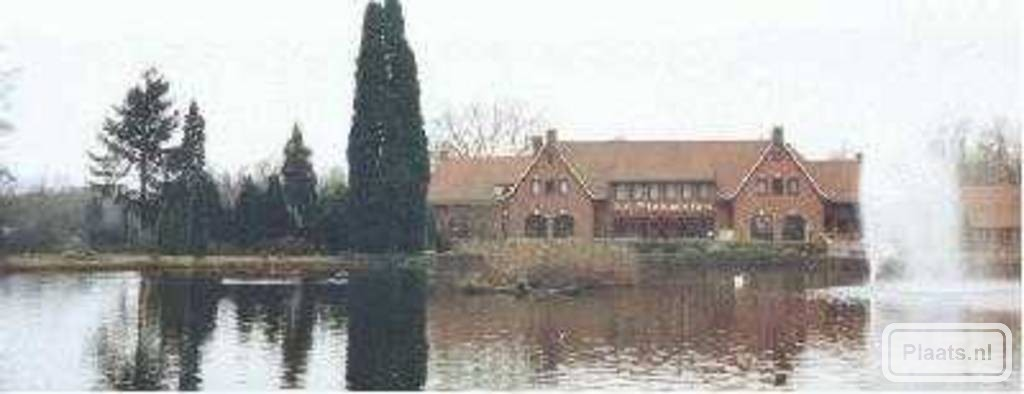
\includegraphics[width=.8\textwidth]{Plasmolen.jpg}
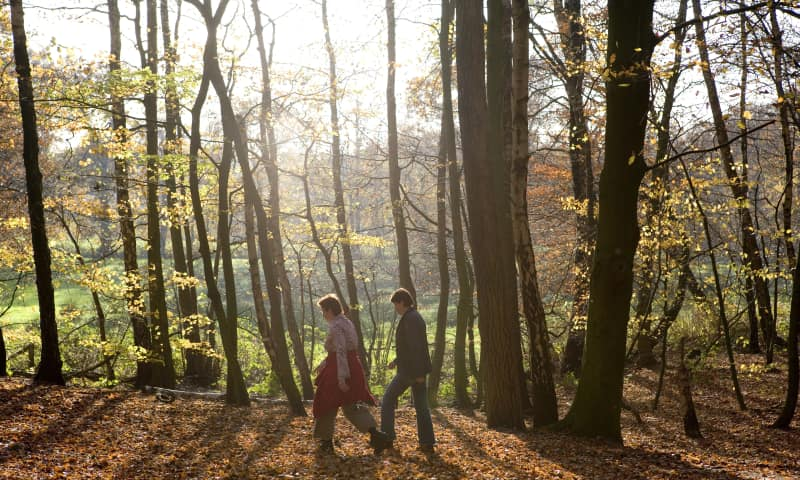
\includegraphics[width=.8\textwidth]{Jansberg.jpg}
\end{center}
}

\frame{
\frametitle{Plasmolen, NL, 1989: REX Workshop on Refinement}

\begin{center}
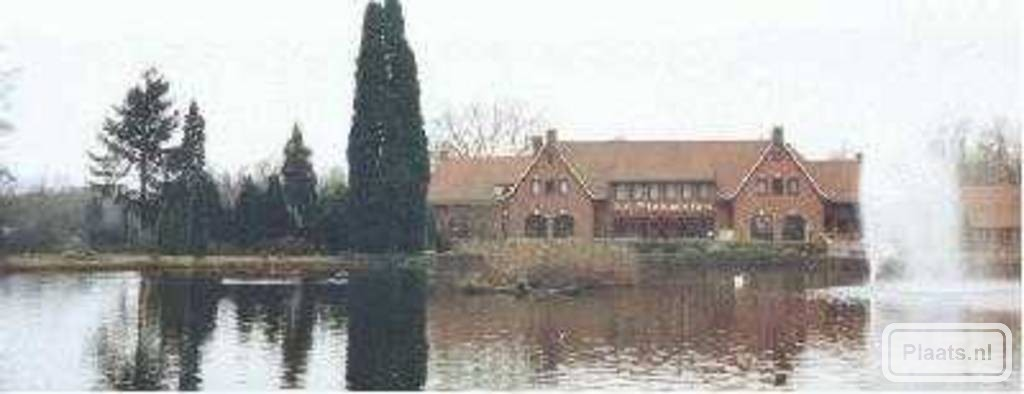
\includegraphics[width=.9\textwidth]{Plasmolen.jpg}
%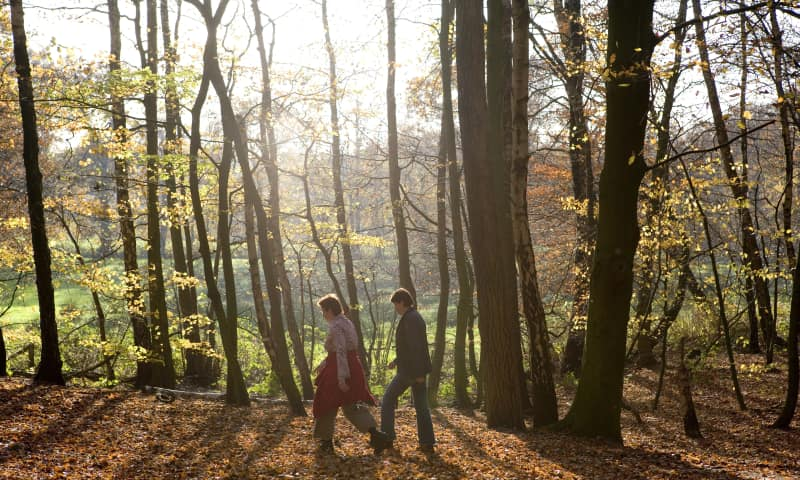
\includegraphics[width=.8\textwidth]{Jansberg.jpg}
\end{center}
}





\frame{
\frametitle{Minimally adequate teacher (Angluin)}

\begin{center}
 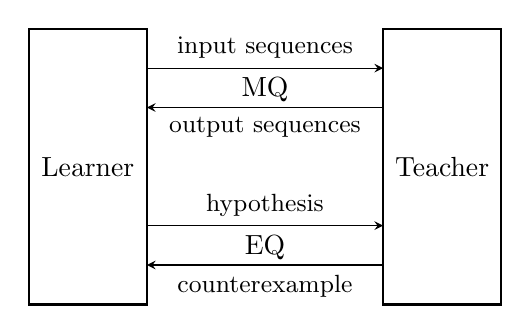
\begin{tikzpicture}[>=stealth]
            \draw [thick] (0,0) rectangle (1.5,3.5) node[midway] {Learner};
            \draw [thick] (4.5,0) rectangle (6,3.5) node[midway] {Teacher};
            \draw [->] (1.5,3) -- (4.5,3) node[midway,below] {MQ};
            \draw (1.5,3) -- (4.5,3) node[midway,above] {\small input sequences};
            \draw [<-] (1.5,2.5) -- (4.5,2.5) node[midway,below] {\small output sequences};
            \draw [->] (1.5,1) -- (4.5,1) node[midway,below] {EQ};
            \draw (1.5,1) -- (4.5,1) node[midway,above] {\small hypothesis};
            \draw [<-] (1.5,0.5) -- (4.5,0.5) node[midway,below] {\small counterexample};
        \end{tikzpicture}
        \hspace{2 em}
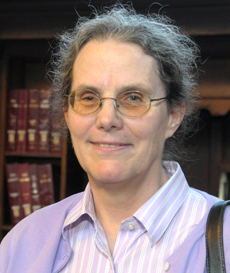
\includegraphics[width=.25\textwidth]{angluin.png}
\end{center}
}
\frame{
\frametitle{Black box checking (Peled, Vardi \& Yannakakis)}

\begin{center}
 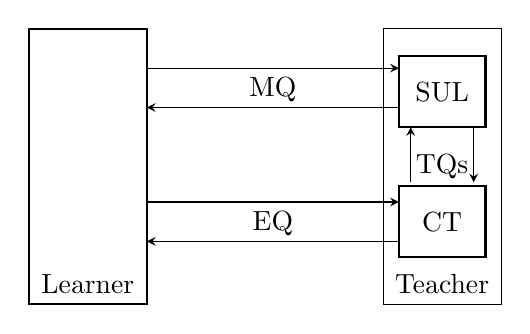
\begin{tikzpicture}[>=stealth]
            \draw [thick] (0,0) rectangle (1.5,3.5);
            \draw (4.5,0) rectangle (6,3.5) node[midway] {TQs};
            \draw [thick] (4.7,2.25) rectangle (5.8,3.15) node[midway] {SUL};
            \draw [thick] (4.7,0.6) rectangle (5.8,1.5) node[midway] {CT};
            \draw [->] (1.5,3) -- (4.7,3) node[midway,below] {MQ};
            \draw [<-] (1.5,2.5) -- (4.7,2.5);
            \draw [->] (1.5,1.3) -- (4.7,1.3) node[midway,below] {EQ};
            \draw [<-] (1.5,0.8) -- (4.7,0.8);
            \draw [->] (4.85,1.55) -- (4.85,2.25);
            \draw [<-] (5.65,1.55) -- (5.65,2.25);
            \node [below] at (0.75,0.5) {Learner};
            \node [below] at (5.25,0.5) {Teacher};
        \end{tikzpicture}
                \hspace{1 em}
        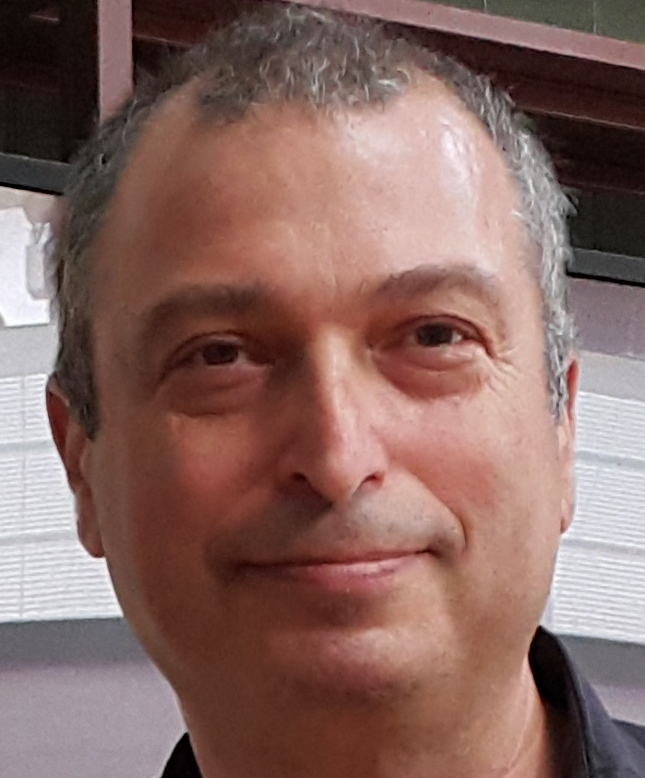
\includegraphics[width=1.2cm]{peled.jpg}
        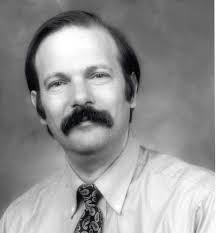
\includegraphics[width=1.35cm]{vardi.jpeg}
        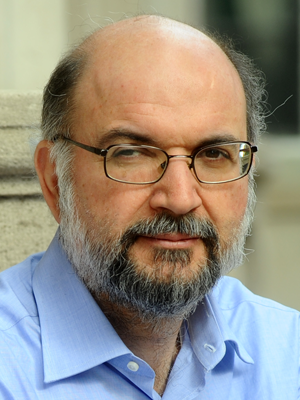
\includegraphics[width=1.1cm]{Yannakakis.png}
\end{center}
\red{Learner}: Formulate hypotheses\\
\red{Conformance Tester (CT)}: Test correctness hypotheses

\pause
\vspace{0.5em}
\red{Model learning and conformance testing two sides of same coin!}
}

\frame{
\frametitle{LearnLib}

\begin{center}
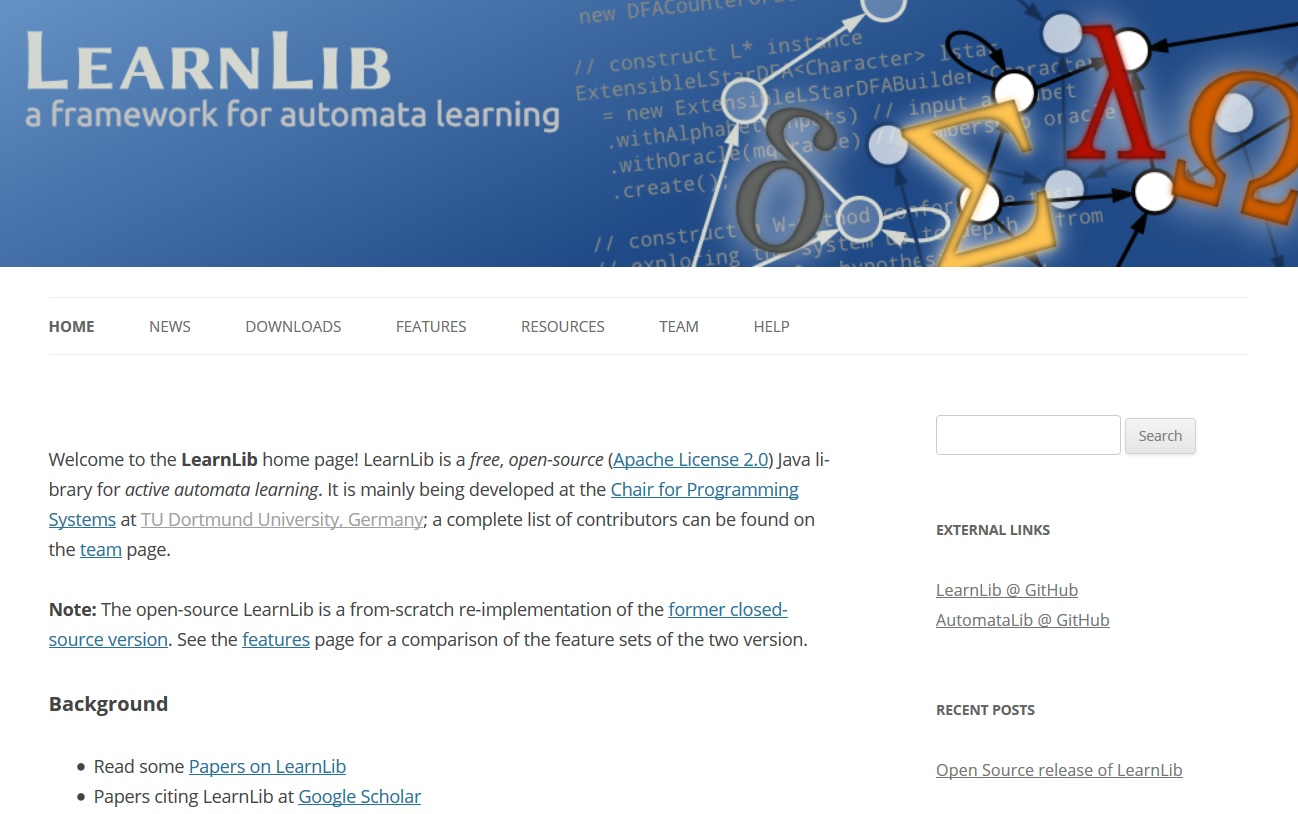
\includegraphics[width=.7\textwidth]{LearnLib.jpg}
    \hspace{1 em}
        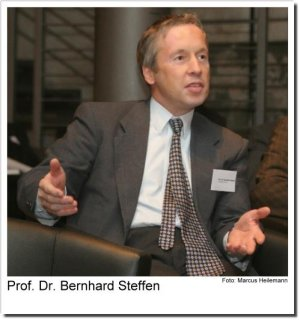
\includegraphics[width=2.5cm]{steffen.jpg}
\end{center}
}


\frame{
\frametitle{Application: E.dentifier2}
\begin{center}
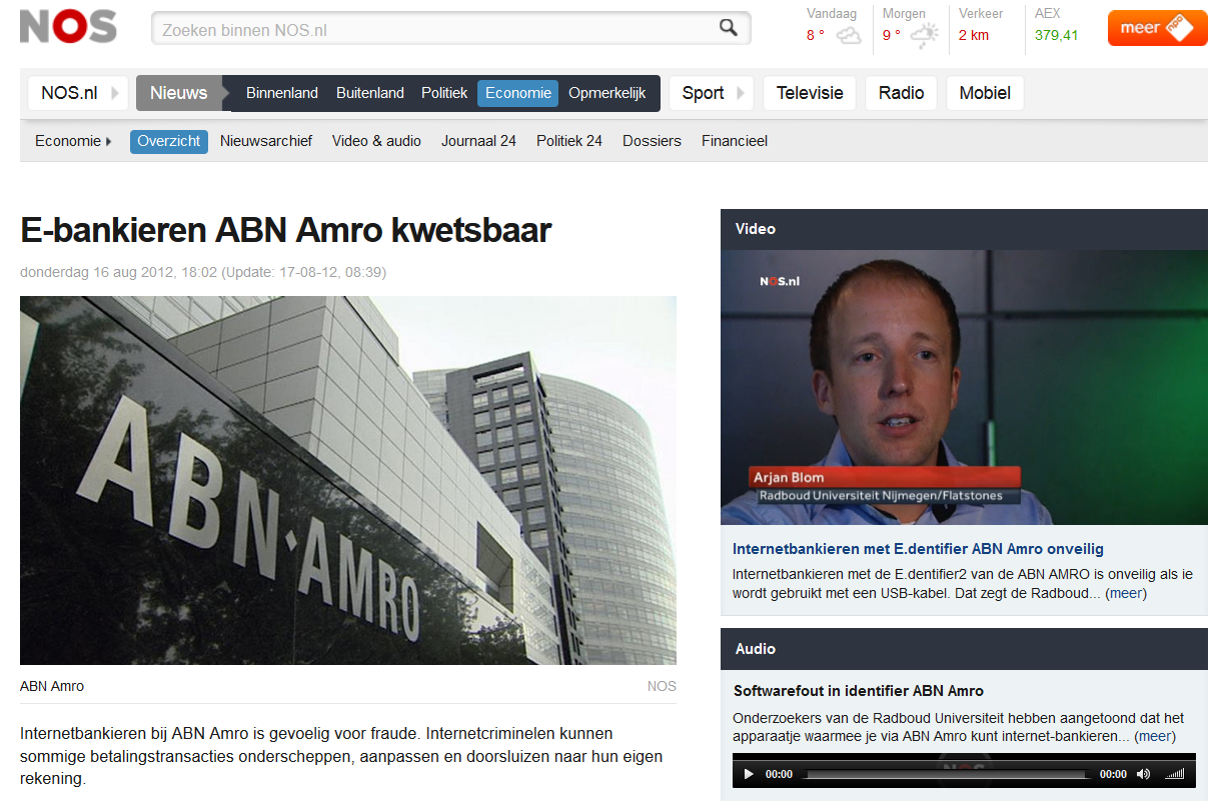
\includegraphics[width=.8\textwidth]{nosedentifier.png}
\end{center}
}

\frame{
\frametitle{State machines for old and new E.dentifier2}
\begin{center}
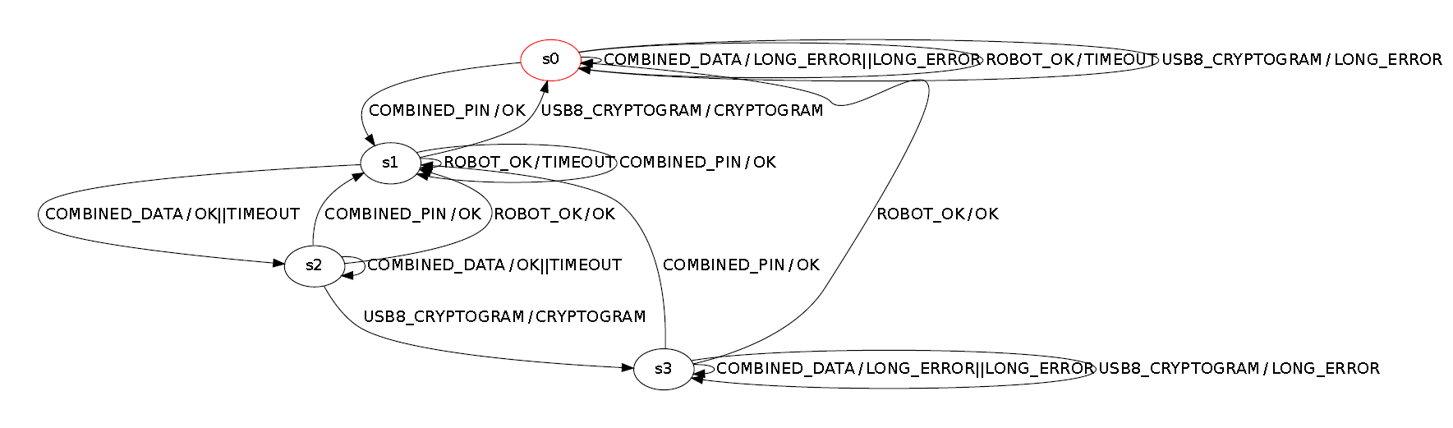
\includegraphics[width=.9\textwidth]{oldedentifier.png}

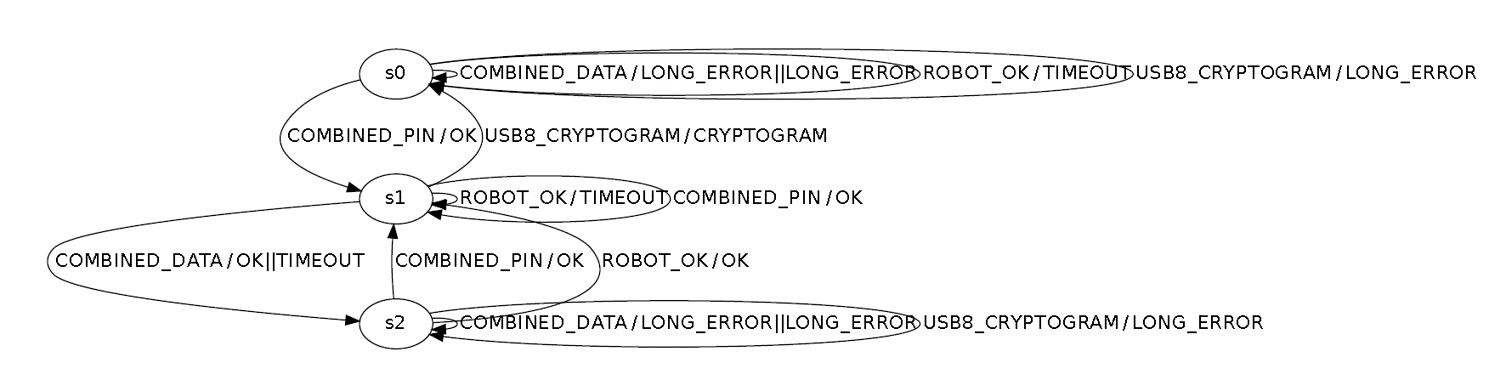
\includegraphics[width=.9\textwidth]{newedentifier.png}
\end{center}
}

\frame{
\frametitle{Bugs in protocol implementations}

\begin{center}
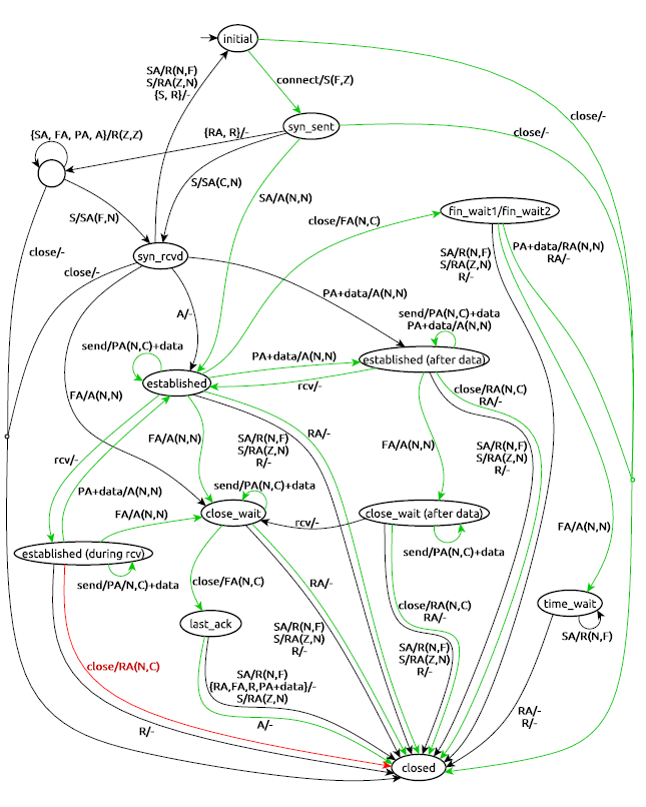
\includegraphics[width=.35\textwidth]{TCPbug.png}
\end{center}
{\small Standard violations found in implementations of major protocols, e.g.,
\blue{TCP}\  (CAV'16, FMICS'17), \blue{TLS}\  (Usenix Security'15), \blue{SSH}\  (Spin'17).}
%
\pause
\red{These findings led to several bug fixes in implementations.}
}

\frame{
\frametitle{Learned model for SSH implementation}

\begin{center}
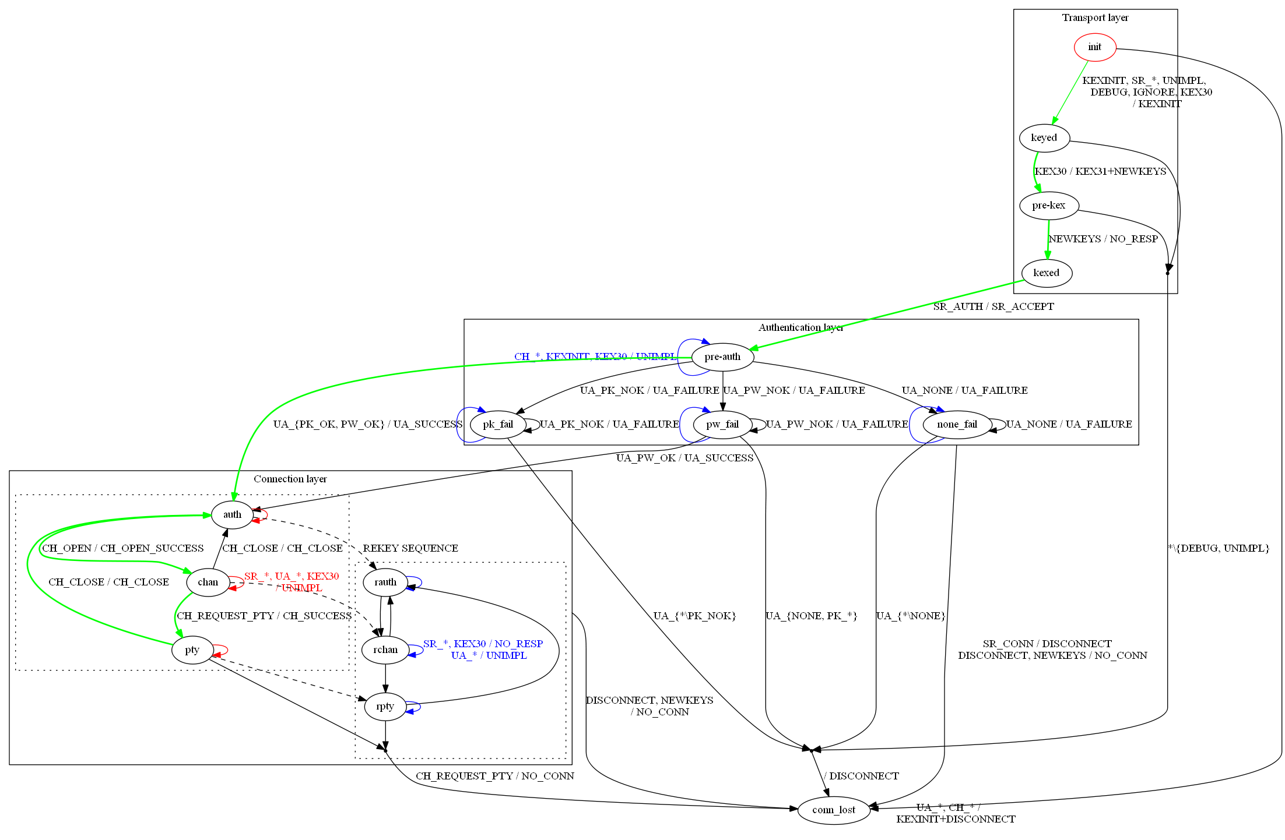
\includegraphics[width=.8\textwidth]{sshbug.png}
\end{center}
}
\frame{
\frametitle{SSH model checking results}

\begin{center}
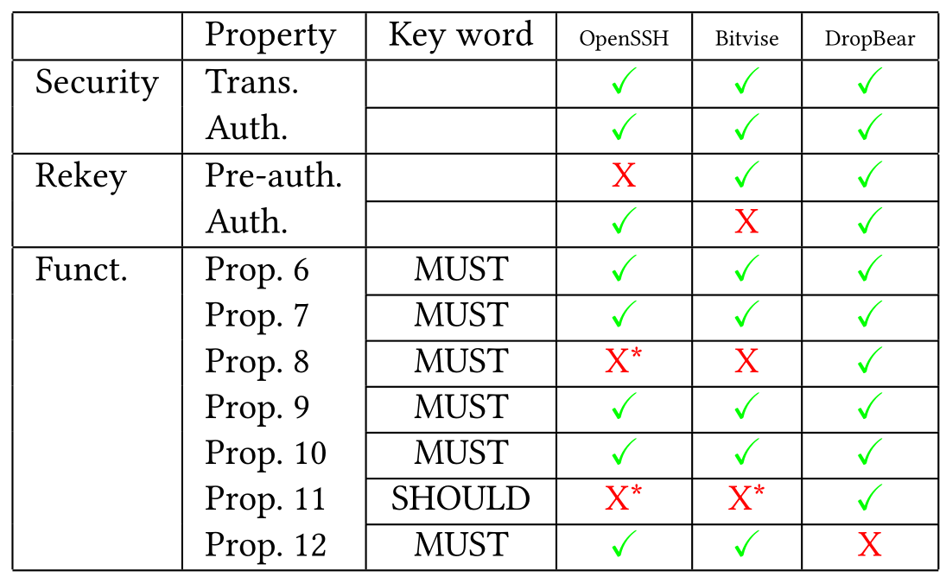
\includegraphics[width=.8\textwidth]{sshresults.png}
\end{center}
}

\frame{
\frametitle{Power Control Service  from Philips Healthcare}

\begin{center}
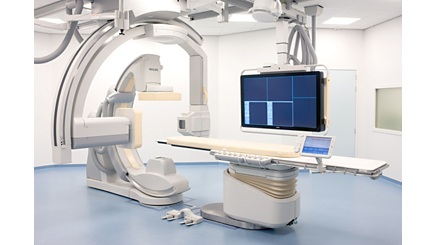
\includegraphics[width=.4\textwidth]{Xray.png}
\end{center}

Are legacy component and refactored implementation equivalent?
}

\frame{
\frametitle{Refactoring Legacy Implementations}

\begin{center}
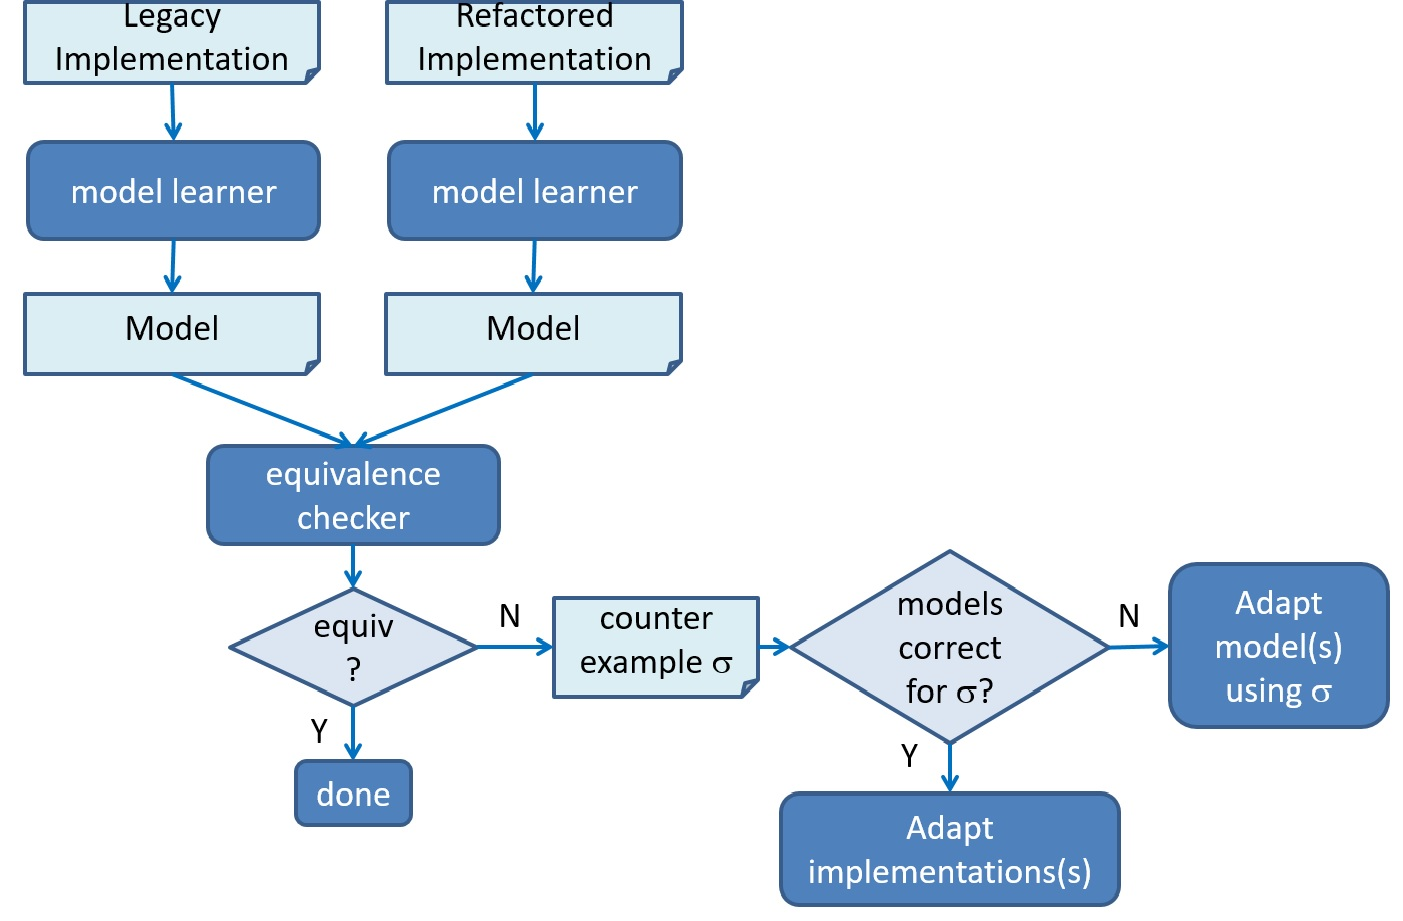
\includegraphics[width=.8\textwidth]{MethodeLegacy.jpg}
\end{center}

\pause
\red{This approach allowed us to find several bugs in refactored implementations.}
}


\frame{
\frametitle{Register Automata}

\begin{center}
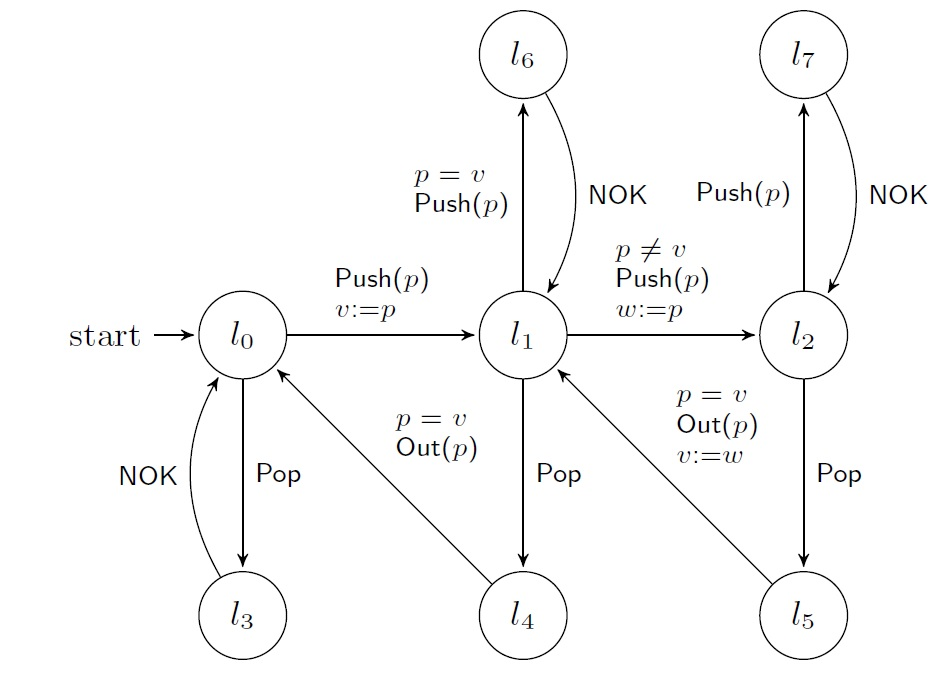
\includegraphics[width=.8\textwidth]{fifoset.jpg}
\end{center}
}

\frame{
\frametitle{Research Problem}

\begin{itemize}
\item 
Model learning is an highly effective bug finding technique
\pause
\item
... but it has some serious scalability problems
\pause
\item
\red{Can we use white-box information while preserving the extensionality of black-box models?}
\end{itemize}
}

\frame{
\frametitle{One Possible Approach: Taint Analysis}

\begin{center}
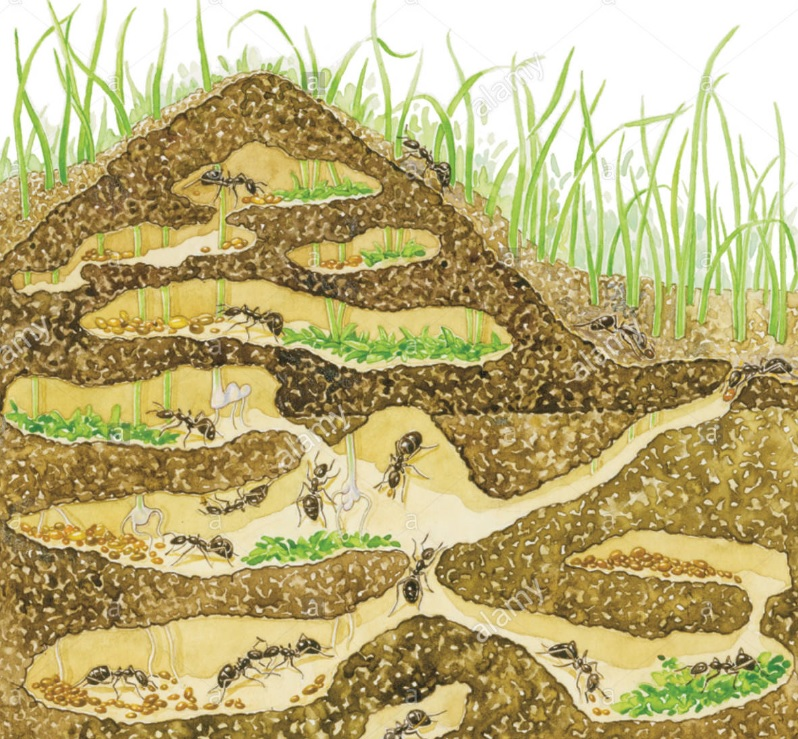
\includegraphics[width=.8\textwidth]{ants.jpg}
\end{center}
}


\frame{
\frametitle{Taint Analysis}

\begin{itemize}
\item
White-box technique for code analysis
\item
Instruments code to track input values
\item
Many tools focus on specific vulnerabilities, e.g.\ buffer overflows and sql injections
\item
Usually implemented using Dynamic Binary Analysis, e.g.\ Valgrind
\item
We use python library from Pygmalion tool from Andreas Zeller et al.
\item
Replace tree oracle in RAlib by a version that uses taint analysis.
\end{itemize}
}

\frame{
\frametitle{What Does Pygmalion Tool Do For Us?}

\begin{center}
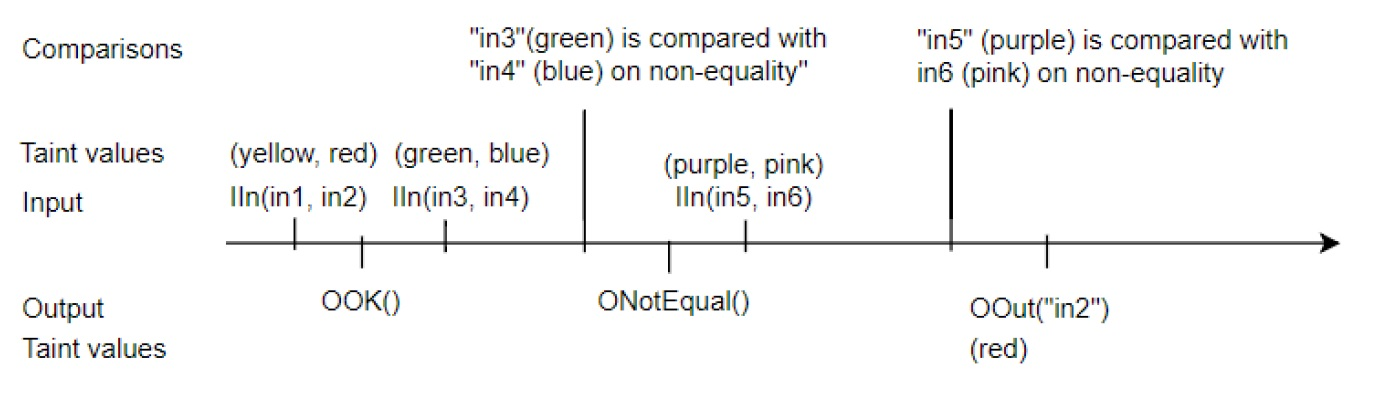
\includegraphics[width=\textwidth]{taintedtrace.jpg}
\end{center}

\pause
\red{Potential of exponential gains during learning!}
}


\frame{
\frametitle{Research Objective}

Our objective is to reach — within say
seven years – the point where model learning and
model based testing have become standard tools in the toolbox
of the software engineer, equally mature as model checking
is right now.

}








\end{document}
